\documentclass{article}
\usepackage[utf8]{inputenc}
\usepackage[italian]{babel}
\usepackage[legalpaper, portrait, margin=1in]{geometry}
\usepackage{setspace}
\onehalfspacing
\usepackage{parskip}
\setlength{\parindent}{0cm}
\usepackage{enumitem}
\setlist{nosep}
\usepackage{hyperref}
\usepackage{graphicx}

\hypersetup{
  	colorlinks,
	citecolor=black,
	filecolor=black,
	linkcolor=black,
	urlcolor=black
}
\title{%
  Olympus DAO Manifiesto \\
  \large DAO funzionale per progetti di cryptovalute opensource }
\author{
  Berrueta, Enrique\\
  \texttt{eabz@polispay.org}
  \and
  Bustos, Ricardo\\
  \texttt{eros@polispay.org}
}
\date{Giugno 2020}

\begin{document}

\maketitle

	\begin{abstract}
	Una DAO è un' ``Organizzazione Autonoma Decentralizzata`` o una corporazione senza un'autorità centrale che può essere governata da un sistema a più parti di membri autorizzati, scelti da una comunità più grande.  Attraverso gli anni, sono stati effettuati molti tentativi di DAO e sistemi di governo, da quando sono state introdotte le cryptovalute. Dalle ``DAO`` di Dash agli Ethereum, tutte queste organizzazioni hanno avuto svariati problemi, a partire dalla mancanza di organizzazione al cadere in una centralizzazione senza diritti. Dopo aver ponderato su quanto esposto, sono arrivato a proporre una nuova soluzione per creare una DAO funzionale, che non sia soltanto decentralizzata, ma anche organizzata e inclusiva.
	\end{abstract}

\newpage

\tableofcontents


\newpage

\section{Struttura}

La DAO sarà basata su cinque pilastri fondamentali, di cui ci sarà una persona in carica scelta dalla comunità, per ogni pilastro:

\begin{itemize}
  \item Tecnologia.
  \item Comunità.
  \item Business.
  \item Adozione.
  \item Marketing.
\end{itemize}

\begin{figure}[h]
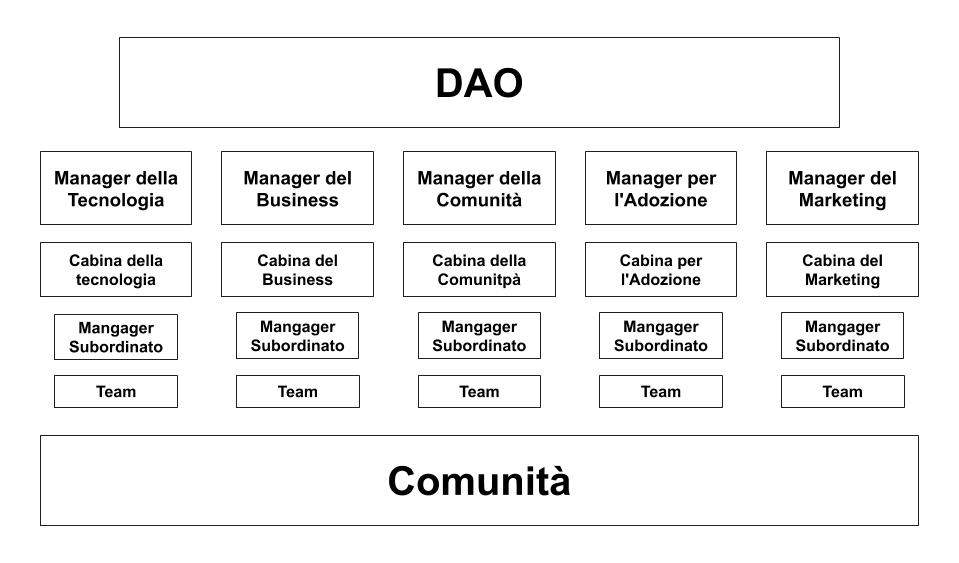
\includegraphics[scale=0.4]{img/dao_structure_it.png}
\centering
\caption{Modello base di organizzazione della DAO}
\end{figure}

Ogni persona in carica, che da ora sarà chiamata ``Manager``, sarà idonea per l'elezione, in base alla sua quota nella DAO. Loro presentaranno una proposta alla comunità, fornendo dettagli sulla loro proposta per il ciclo di comando, che durerò da 6 mesi a un anno, a seconda di quanto deciso dalla comunità. Nella loro proposta, ogni manager della DAO dovrà delineare i seguenti punti:

\begin{itemize}
  \item Proposte di miglioramento.
  \item Membri del loro team (cabina).
  \item Strategie che impiegheranno per raggiungere i loro obiettivi.
  \item Perchè la comunità dovrebbe votare per loro.
  \item Tabella di marcia dettagliata con specifiche tabelle temporali.
\end{itemize}

I manager della DAO potranno essere scelti per la rielezione per tutte le volte che vogliono, finchè la comunità sarò d'accordo con loro.

\section{Chiavi}

Finchè l'intera DAO è riferita a un ecosistema di cryptovalute, tutto ciò che si riferisce al voto e alla presa di decisioni dovrebbe essere effettuato attraverso una chiave DAO. Queste chiavi sono rese sicure dal manager e l'accesso è garantito/rimosso durante il ciclo di votazione DAO, o l'esecuzione di un meccanismo di sicurezza.

Queste chiavi vengono cambiate durante i cicli DAO se il ruolo di un manager cambia in un ciclo di voto o per un meccanismo di sicurezza. Questa Chiave sarà quella che riceve le monete per l'area specifica e sarà usata per sbloccare le monete (assieme agli altri 5 manager) nelle proposte della comunità e in caso di budget sforato.

\section{Piattaforma}

La piattaforma per interagire, votare, proporre alla DAO è la blockchain Olympus.

Ogni utente è in grado di controllare le informazione della DAO, in tempo reale, verificate da un nodo.

Il portafoglio Olympus è la principale piattaforma che gli utenti dovrebbero usare quotidianamente per le funzioni della DAO 

\section{Tesoreria}

Una DAO per funzionare correttamente come un'organizzazione è totalmente richesto di avere dei fondi. Se non è possibile supportarla in base a donazioni, proponiamo un modello di finanziamento che garantisca i fondi equamente e un modello di distribuzione per ogni area. 

Il 20\% delle monete emesse mensilmente verrà bloccato in un account usato per la DAO

Questi fondi verranno distribuiti in tre categorie:

\begin{itemize}
  \item 10\% alle aree DAO.
  \item 5\% per le proposte della comunità.
  \item 5\% bloccati per le aree che sforano il budget.
\end{itemize}

Le aree del budget DAO saranno distribuite in base alle seguenti proporzioni:

\begin{itemize}
  \item 30\% Tecnologia.
  \item 10\% Comunità.
  \item 20\% Business.
  \item 20\% Marketing.
  \item 20\% Adozione.
\end{itemize}

Il 5\% per le proposte della comunità dovrebbe essere distribuito in base aile decisioni dei Manager DAO. Loro decideranno quando una proposta dovrebbe essere finanziata.

Il 5\% per le aree che sforano il budget dovrebbe essere usato in base alla decisione dei Manager DAO per incrementaer una specifica area di budget per uno specifico periodo.

I fondi saranno depositati ogni mese alal Chiave manager corrente, in automatico dalla rete.

La comunità e le aree con budget sforato riceveranno depositi in una chiave multifirma generata, per assicurare che solo 3 su 5 manager siano in grado di prelevare questi fondi.
Se un manager non carica il rapport alla rete, la sua chiave è automaticamente rimossa dalle chiavi DAO.

Le proposte della comunitò devono specificare:

\begin{itemize}
  \item Quantità di budget necessario.
  \item Piano d'azione.
  \item Dettagli costi del budget.
\end{itemize}

\section{Cicli}

La funzionalità della DAO è determinata da cicli temporali. Ci sono solo tre cicli temporali che implicano decisioni in momenti diversi.

\subsection{Ciclo di votazione}

Il ciclo di voto inizia  ogni anno il 20 gennaio. QUesto processo impiega circa 2 o 3 settimane e l'idea è di avere una campagna elettorale in cui i vecchi Manager DAO e i nuovi memberi che vogliono essere coinvolti tecnicamente nella DAO devono creare le loro proposte e tabelle di marcia per essere qualificati.

Questo ciclo ha quattro fasi:

\begin{itemize}
  \item Postulazione dei candidati.
  \item Proposte dei candidati.
  \item Preparazione delle elezioni.
  \item Votazione.
\end{itemize}

\subsection{Ciclo del Budget}

QUando i Membri DAO evngono scelti devino fornire un budget adeguato che opererà nei successivi tre mesi. QUesto budget dovrebbe essere presentato dal Business Manager DAO ogni tre mesi, includendo il budget e le spese reali, per fornire alla comunità un'informazione trasparente.

\subsection{Ciclo di Report}

Assieme ai cicli di Budget, ogni DAO Manager dovrebbe creare un report sulle proprie aree, riguardo gli obiettivi del lavoro di 3 mesi, al Manager DAO e alla comunitò.

I fondi saranno depositati ogni mese alal Chiave manager corrente, in automatico dalla rete.

\section{Aree}

\subsection{Tecnologia}

Il manager DAO in carica alla tecnologia sarà responsabile di trovare e istruire sviluppatori per seguire la tabella di marcia tecnica della DAO.

Il manager avrà i seguenti compiti:

\begin{itemize}
  \item Sviluppo tecnologico della criptovaluta.
  \item Sviluppo casi d'utilizzo.
  \item Librerie di terze parti.
  \item Documentazione e mantenimento.
\end{itemize}

Accanto, il manager della comunità in carica del corretto funzionamento e documentazione dei seguenti servizi:

\begin{itemize}
  \item Esploratore di blocchi ufficiale.
  \item Siti Websites.
  \item Guide.
  \item Forum di discussione.
  \item Risorse interne.
\end{itemize}

\subsection{Comunità}

Il manager DAO in carica alla comunità sarà responsabile per essa e per l'integrità e la correttezza dell'informazione mostrata in diversi canali. 

Il manager avrà le seguenti responsabilità:

\begin{itemize}
  \item Comunicazione e social media.
  \item Documentazione e mantenimento.
  \item Supporto tecnico per gli utenti e migliori pratiche di sicurezza.
  \item Branding e design corretti.
\end{itemize}

Accanto, il manager della comunità in carica del corretto funzionamento e documentazione dei seguenti servizi:

\begin{itemize}
  \item Esploratore di blocchi ufficiale.
  \item Siti Websites.
  \item Guide.
  \item Forum di discussione.
  \item Risorse interne.
\end{itemize}

\subsection{Business}

Il manager DAO in carica per il business + responsabile di stabilire nuove partnership con altri progetti e seguire le proposte della comunità.

Il manager avrà le seguenti responsabilità:

\begin{itemize}
  \item Partnership.
  \item Amministrazione e trasparenza del budget.
  \item Proposte della comunità da seguire.
\end{itemize}

\subsection{Adozione}

Il manager DAO in carica per l'adozione sarà responsabile per portare nuovi commercianti nel progetto e di portare nuovi sviluppatori per usare la tecnologia per i propri scopi e organizzare eventi per attrarre l'utilizzo della rete.

Il manager avrà i seguenti compiti:

\begin{itemize}
  \item Adozione commerciale.
  \item Adozione sviluppatori.
  \item Relazioni pubbliche e ufficio informativo.
\end{itemize}

\subsection{Marketing}

Il manager in carica al marketing sarà responsabile per il raggiungimento di nuovi spazi e di fornire agli altri manager analisi e strategie di marketing.

Il manager avrà i seguenti compiti:

\begin{itemize}
  \item Strategie di marketing e tabelle di marcia.
  \item Rapporti d'analisi e di intelligence.
  \item Spazi pubblicitari.
\end{itemize}

\section{Meccanismi di Sicurezza}

Visto che la DAO implica la fiducia dell'organizzazione a membri conosciuti, i meccanismi di sicurezza dovrebbero essere sviluppati in base alla discussione e la sicurezza della rete. 

Abbiamo pensato a due casi differenti in cui un problema può accadere nella struttura della DAO od ai fondi. Per coprire questi due casi abbiamo creato il seguente meccanismo di sicurezza.

\subsection{Interdizione dei Manager}

Se sotto ogni circostanza i Manager DAO vogliono rimuovere un membro, possono usare la loro Chiave DAO per creare un messaggio firmato per la rete al fine di rimuovere la chiave dalle Chiavi DAO. Per l'esecuzione di questo meccanismo sono necessarie almeno 3-5 possibili firme.

\subsection{Interdizione DAO}

Questo meccanismo è eseguito dalla comunità, e implica che i Manager DAO in qualche modo non facciano il loro lavoro correttamente o che l'intera DAO sia gestita da un gruppo che danneggia l'intero ecosistema. 

I membri della comunità possono creare un messaggio firmato che include una "prova di possesso" di un numero di monete, una volta che la soglia supera il 30\% della fornitura totale di moneta, tutte le chiavi DAO vengono rimosse e un ciclo di voto di emergenza inizia.

\end{document}
